\documentclass{beamer}

\usepackage[utf8]{inputenc}
\usepackage{braket}

\title{Practical Byzantine Fault Tolerance}
\subtitle{Apresentação para a disciplina MATA88}
\author{Gabriel Dahia, Pedro Vidal}
\date{21 de Fevereiro de 2018}
\institute{Universidade Federal da Bahia}

\begin{document}

\frame{\maketitle}

\begin{frame}
  \frametitle{Introdução}
  \framesubtitle{Problema}

  \begin{itemize}
    \item
      Aumento da dependência de serviços online - ataques maliciosos;

      \pause
    \item
      Complexidade do software crescente causa erros;

      \pause
    \item
      Ataques maliciosos e erros ocasionam falhas bizantinas.
  \end{itemize}
\end{frame}

\begin{frame}
  \frametitle{Introdução}
  \framesubtitle{Contribuição}

  Um algoritmo prático para replicação de máquina de estados que tolera falhas bizantinas:
  \begin{itemize}
      \pause
    \item
      Garante \textit{liveness} e \textit{safety};

      \pause
    \item
      Funciona em sistemas assíncronos*;

      \pause
    \item
      Não depende de sincronia para \textit{safety};
      
      \pause
    \item
      Performance superior à métodos anteriores;

      \pause
    \item
      Descreve otimizações que permitem uso prático.
  \end{itemize}
\end{frame}

\begin{frame}
  \frametitle{Modelo do Sistema}
  \framesubtitle{Comunicação}

  \begin{itemize}
    \item
      Sistema distribuído assíncrono;
      
      \pause
    \item
      Nós são conectados por rede que pode:
      \begin{itemize}
        \item
          falhar em entregar mensagens;

        \item
          atrasá-las;

        \item
          duplicá-las; ou

        \item
          entregá-las fora de ordem.
      \end{itemize}
  \end{itemize}

\end{frame}

\begin{frame}
  \frametitle{Modelo do Sistema}
  \framesubtitle{Falhas}

  \begin{itemize}
    \item
      Modelo de falhas bizantinas;
      
    \item
      Exceção - nós falham independentemente:
      \begin{itemize}
          \pause
        \item
          implementações diferentes por dispositivo;

          \pause
        \item
          sistemas operacionais diversos; e

          \pause
        \item
          senhas e administradores distintos.
      \end{itemize}
  \end{itemize}
\end{frame}

\begin{frame}
  \frametitle{Modelo do Sistema}
  \framesubtitle{Segurança}

  \begin{itemize}
    \item
      Criptografia para prevenir \textit{spoofing}, \textit{replays} e detecção de mensagens corrompidas;

    \item
      Técnicas que com alta probabilidade não podem ser subvertidas:
      \begin{itemize}
        \item
          Assinaturas de chave-pública;
          
        \item
          Códigos de autenticação; e
          
        \item
          Sumário de mensagens.
      \end{itemize}
  \end{itemize}
\end{frame}

\begin{frame}
  \frametitle{Modelo do Sistema}
  \framesubtitle{Adversário}

  \begin{itemize}
      \item
        Coordena nós comprometidos;

      \pause
      \item
        Atrasa comunicação;

      \pause
      \item
        Atrasa nós corretos não-indefinidamente.
  \end{itemize}
\end{frame}

\begin{frame}
  \frametitle{Propriedades do Serviço}

  \begin{itemize}
    \item
      Implementa qualquer serviço replicado com um \textbf{estado} e algumas \textbf{operações};

      \pause
    \item
      Computações deterministícas arbitrárias;

      \pause
    \item
      Clientes fazem requisições de invocação e bloqueiam esperando por uma resposta;

      \pause
    \item
      Clientes e réplicas são corretos se seguem o algoritmo e suas assinaturas estão protegidas.
  \end{itemize}
\end{frame}

\begin{frame}
  \frametitle{Propriedades do Serviço}
  \framesubtitle{Resiliência ótima}

  \begin{figure}
    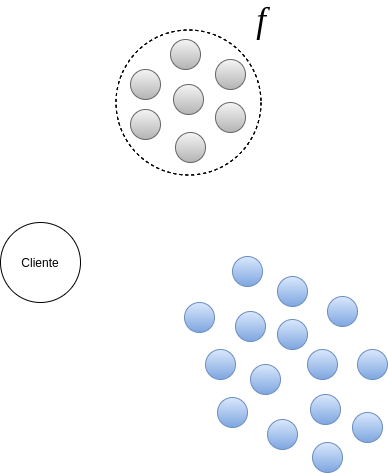
\includegraphics[width=0.5\textwidth]{images/resiliencia01}<1>
    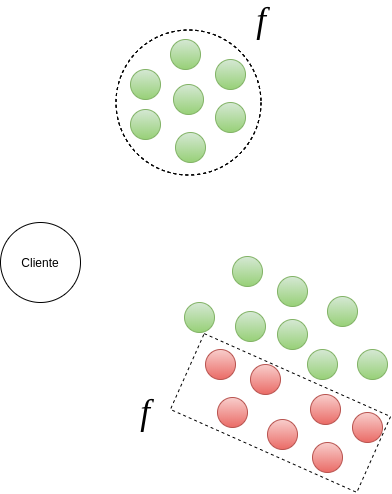
\includegraphics[width=0.51\textwidth]{images/resiliencia02}<2>
    \caption{Cliente faz requisição}
  \end{figure}

\end{frame}

\begin{frame}
  \frametitle{Propriedades do Serviço}
  \framesubtitle{\textit{Safety}}

  Funciona como se centralizado, executando operações atomicamente, uma por vez.
  \begin{itemize}
      \pause
    \item
      Depende do número de réplicas que falham;

      \pause
    \item
      Não depende de sincronia;

      \pause
    \item
      Independe do número de clientes comprometidos;

      \pause
    \item
      Não é protegido contra clientes maliciosos:
      \pause
      \begin{itemize}
        \item
          Controle de acesso mitiga o problema.
      \end{itemize}
  \end{itemize}
\end{frame}

\begin{frame}
  \frametitle{Propriedades do Serviço}
  \framesubtitle{\textit{Liveness}}

  Cliente eventualmente recebe resposta.
  \begin{itemize}
      \pause
    \item
      Depende de sincronia e retransmissões;
      
      \pause
    \item
      Sincronia fraca: atraso não cresce mais rápido do que linearmente.
  \end{itemize}
\end{frame}

\begin{frame}
  \frametitle{Algoritmo}
  \framesubtitle{Definições}

  \begin{itemize}
    \item
      Máquina de estados replicada pelos processos;

      \pause
    \item
      Cada réplica mantém o estado e implementa operações;

      \pause
    \item
      Conjunto de réplicas $\mathcal{R}$, numeradas $0, ..., |\mathcal{R}| - 1$;

      \pause
    \item
      $|\mathcal{R}| = 3f + 1$.
  \end{itemize}
\end{frame}

\begin{frame}
  \frametitle{Algoritmo}
  \framesubtitle{Definições}

  \begin{itemize}
    \item
      Sistema tem \textbf{visões}, $v$, consecutivas;

    \item
      Réplicas são:
      \begin{itemize}
        \item
          \textbf{primária} - se $p = v \text{ mod } |\mathcal{R}|$; ou
          
        \item
          \textbf{backups}.
      \end{itemize}

    \item
      Visão muda quando primária for suspeita.
  \end{itemize}
\end{frame}

\begin{frame}
  \frametitle{Algoritmo}
  \framesubtitle{Funcionamento}

  \begin{figure}
    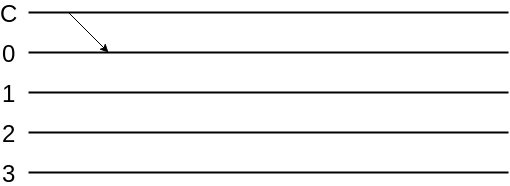
\includegraphics[width=0.75\textwidth]{images/algo01}<1>
    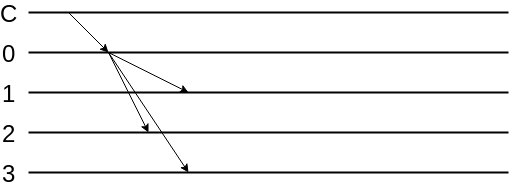
\includegraphics[width=0.75\textwidth]{images/algo02}<2>
    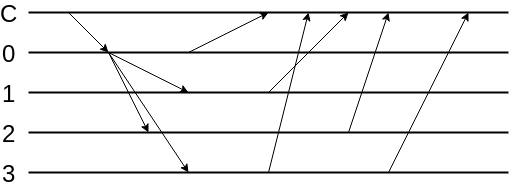
\includegraphics[width=0.75\textwidth]{images/algo03}<3>
    \caption{Esboço do funcionamento do algoritmo}
  \end{figure}
\end{frame}

\begin{frame}
  \frametitle{Algoritmo}
  \framesubtitle{Funcionamento}

  \begin{itemize}
    \item
      Réplicas precisam:
      \begin{itemize}
        \item
          ser determinísticas;

        \item
          começar no mesmo estado.
      \end{itemize}

    \item
      Todas as réplicas concordam em ordem total para execução, apesar de falhas.
  \end{itemize}
\end{frame}

\begin{frame}
  \frametitle{Algoritmo}
  \framesubtitle{Cliente}

  \begin{figure}
    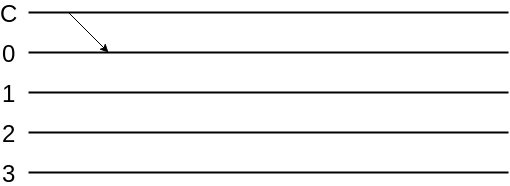
\includegraphics[width=0.75\textwidth]{images/algo01}
    \only<1>{\caption{Envia $\braket{\text{REQUEST}, o, t, c}{}_{\sigma_c}$}}
    \only<2>{\caption{Envia $\braket{\text{REQUEST}, \text{\alert{$o$}}, t, c}{}_{\sigma_c}$}}
    \only<3>{\caption{Envia $\braket{\text{REQUEST}, o, \text{\alert{$t$}}, c}{}_{\sigma_c}$}}
    \only<4>{\caption{Envia $\braket{\text{REQUEST}, o, t, \text{\alert{$c$}}}{}_{\text{\alert{$\sigma_c$}}}$}}
  \end{figure}
\end{frame}

\begin{frame}
  \frametitle{Algoritmo}
  \framesubtitle{Cliente}

  \begin{figure}
    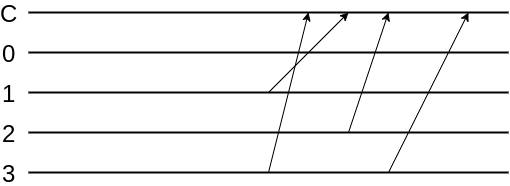
\includegraphics[width=0.75\textwidth]{images/client02}
    \only<1>{\caption{Réplicas respondem $\braket{\text{REPLY}, v, t, c, i, r}{}_{\sigma_i}$}}
    \only<2>{\caption{Réplicas respondem $\braket{\text{REPLY}, \text{\alert{$v$}}, t, c, i, r}{}_{\sigma_i}$}}
    \only<3>{\caption{Réplicas respondem $\braket{\text{REPLY}, v, \text{\alert{$t$}}, c, i, r}{}_{\sigma_i}$}}
    \only<4>{\caption{Réplicas respondem $\braket{\text{REPLY}, v, t, \text{\alert{$c$}}, i, r}{}_{\sigma_i}$}}
    \only<5>{\caption{Réplicas respondem $\braket{\text{REPLY}, v, t, c, \text{\alert{$i$}}, r}{}_{\text{\alert{$\sigma_i$}}}$}}
    \only<6>{\caption{Réplicas respondem $\braket{\text{REPLY}, v, t, c, i, \text{\alert{$r$}}}{}_{\sigma_i}$}}
  \end{figure}
\end{frame}

\begin{frame}
  \frametitle{Algoritmo}
  \framesubtitle{Cliente}

  \begin{figure}
    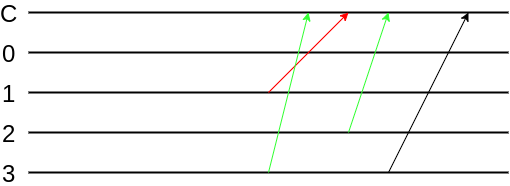
\includegraphics[width=0.75\textwidth]{images/client03}
    \caption{Cliente espera por $f+1$ respostas $\braket{\text{REPLY}, v, \text{\color{green} $t$}, c, i, \text{\color{green} $r$}}{}_{\sigma_i}$}
  \end{figure}
\end{frame}

\begin{frame}
  \frametitle{Algoritmo}
  \framesubtitle{Cliente}

  \begin{figure}
    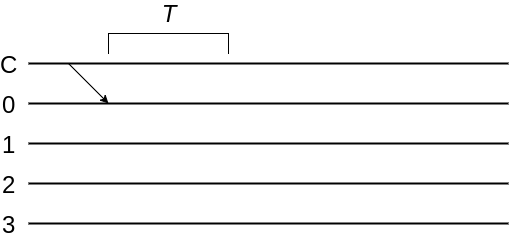
\includegraphics[width=0.75\textwidth]{images/client04}<1>
    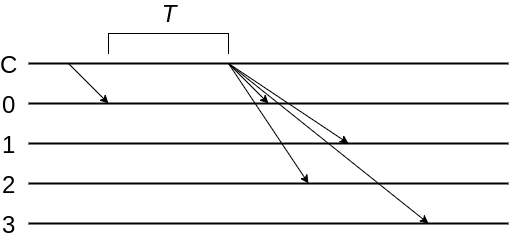
\includegraphics[width=0.75\textwidth]{images/client05}<2>
    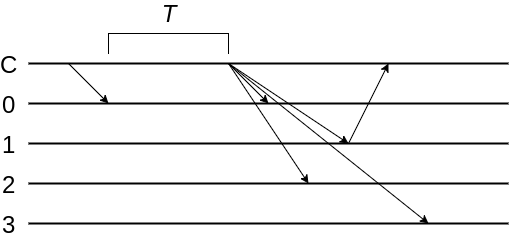
\includegraphics[width=0.75\textwidth]{images/client06}<3>
    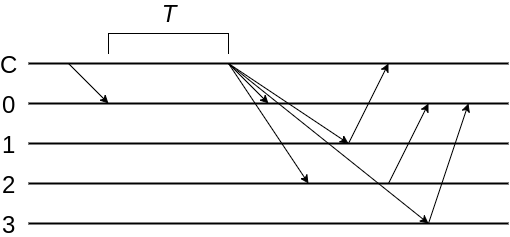
\includegraphics[width=0.75\textwidth]{images/client07}<4->
    \only<1>{\caption{Cliente dá \textit{timeout} esperando $f+1$ respostas}}
    \only<2>{\caption{Cliente faz \textit{broadcast} da requisição a todas as réplicas}}
    \only<3>{\caption{Réplicas que já tem $r$ reenviam ao cliente}}
    \only<4>{\caption{\textit{Backups} que ainda não tem, enviam requisição à primária}}
    \only<5>{\caption{Se primária não repassar ao grupo, será suspeita e visão mudará}}
  \end{figure}
\end{frame}

\begin{frame}
  \frametitle{Algoritmo}
  \framesubtitle{Operação Normal}

  \begin{itemize}
    \item
      Estado da réplica inclui:
      \begin{itemize}
        \item
          estado do serviço;

        \item
          \textit{log} de mensagens;

        \item
          visão atual $v$.
      \end{itemize}
  \end{itemize}
\end{frame}

\begin{frame}
  \frametitle{Algoritmo}
  \framesubtitle{Operação Normal}

  \begin{itemize}
    \item
      Protocolo de repasse de requisição em 3 fases:
      \begin{itemize}
        \item
          pré-preparação - ordenação de requisições;

        \item
          preparação - ordenação de requisições e garantia de ordenação entre visões;

        \item
          \textit{commit} - garantia de ordenação entre visões.
      \end{itemize}
  \end{itemize}
\end{frame}

\begin{frame}
  \frametitle{Algoritmo}
  \framesubtitle{Operação Normal}

  \begin{figure}
    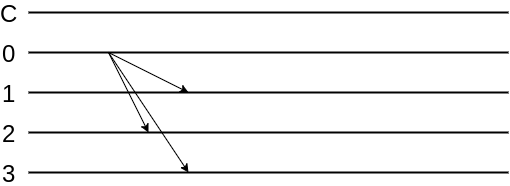
\includegraphics[width=0.75\textwidth]{images/preprepare}
    \only<1>{\caption{Primária envia $\braket{\braket{\text{PRE-PREPARE}, v, n, d}_{\sigma_p}{}, m}{}$}}
    \only<2>{\caption{Primária envia $\braket{\braket{\text{PRE-PREPARE}, v, \text{\alert{$n$}}, d}_{\sigma_p}{}, m}{}$}}
    \only<3>{\caption{Primária envia $\braket{\braket{\text{PRE-PREPARE}, v, n, \text{\alert{$d$}}}_{\sigma_p}{}, m}{}$}}
    \only<4>{\caption{Primária envia $\braket{\braket{\text{PRE-PREPARE}, v, n, d}_{\sigma_p}{}, \text{\alert{$m$}}}{}$}}
  \end{figure}
\end{frame}

\begin{frame}
  \frametitle{Algoritmo}
  \framesubtitle{Operação Normal}

  \textit{Backup} aceita $\braket{\text{PRE-PREPARE}, v, n, d}{}_{\sigma_p}$, e adiciona ao log, se:
  \begin{itemize}
    \item
      $\sigma_p$ é válida;
      
      \pause
    \item
      $d = D(m)$;

      \pause
    \item
      Sua visão é $v$;

      \pause
    \item
      Não aceitou outra mensagem de pré-preparação na visão $v$ e número $n$ com sumário diferente;

      \pause
    \item
      $h < n < H$.
  \end{itemize}
\end{frame}

\begin{frame}
  \frametitle{Algoritmo}
  \framesubtitle{Operação Normal}

  \begin{figure}
    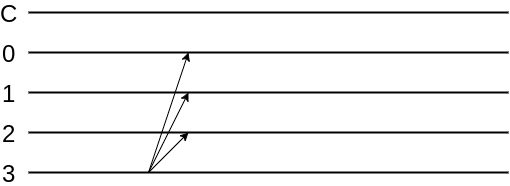
\includegraphics[width=0.75\textwidth]{images/prepare}
    \caption{Fase de preparação, envio de $\braket{\text{PREPARE}, v, n, d, i}{}_{\sigma_i}$}
  \end{figure}
\end{frame}

\begin{frame}
  \frametitle{Algoritmo}
  \framesubtitle{Operação Normal}

  Réplica aceita $\braket{\text{PREPARE}, v, n, d, i}{}_{\sigma_i}$, e adiciona ao log, se:
  \begin{itemize}
    \item
      $\sigma_i$ é válida;

    \item
      Sua visão é $v$;

    \item
      $h < n < H$.
  \end{itemize}
\end{frame}

\begin{frame}
  \frametitle{Algoritmo}
  \framesubtitle{Operação Normal}

  $\texttt{prepared}(m, v, n, i)$ sse a réplica $i$ inseriu em seu log:
  \begin{itemize}
      \pause
    \item
      A requisição $m$;

      \pause
    \item
      Uma mensagem de pré-preparação para $m$ na visão $v$ de número $n$; e

      \pause
    \item
      $2f$ mensagens distintas de preparação válidas.
  \end{itemize}
\end{frame}

\begin{frame}
  \frametitle{Algoritmo}
  \framesubtitle{Operação Normal}

  \begin{block}{Invariante (1)}
    Se $$\texttt{prepared}(m, v, n, i),$$ então $$\forall j \forall m' (D(m') \neq D(m) \to \lnot \texttt{prepared}(m', v, n, j)).$$
  \end{block}

  Razão:
  \begin{itemize}
      \pause
    \item
      Se $\texttt{prepared}(m, v, n, i)$, então $f + 1$ réplicas corretas enviaram mensagens de pré-preparação ou preparação;

      \pause
    \item
      Para $\texttt{prepared}(m', v, n, j)$, precisamos de $j$ e $2f$ mensagens distintas de preparação válidas;

      \pause
    \item
      Mas $f + 1$ já se comprometeram com $m, v, n$;
      
      \pause
    \item
      Logo, $|\mathcal{R}| = 3f + 1 < 2f + (f + 1) + |\{j\}|$.
  \end{itemize}
\end{frame}

\begin{frame}
  \frametitle{Algoritmo}
  \framesubtitle{Operação Normal}

  \begin{figure}
    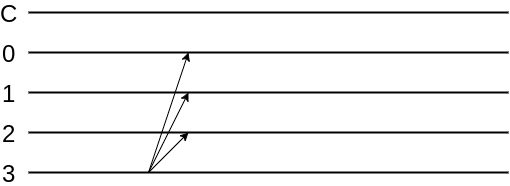
\includegraphics[width=0.75\textwidth]{images/prepare}
    \only<1>{\caption{$\texttt{prepared}(m, v, n, i)$ indica começo da fase de \textit{commit}}}
    \only<2>{\caption{Envio de $\braket{\text{COMMIT}, v, n, D(m), i}{}_{\sigma_i}$}}
  \end{figure}
\end{frame}

\begin{frame}
  \frametitle{Algoritmo}
  \framesubtitle{Operação Normal}

  Réplica aceita $\braket{\text{COMMIT}, v, n, D(m), i}{}_{\sigma_i}$, e adiciona ao log, se:
  \begin{itemize}
    \item
      $\sigma_i$ é válida;

    \item
      Sua visão é $v$;

    \item
      $h < n < H$.
  \end{itemize}
\end{frame}

\begin{frame}
  \frametitle{Algoritmo}
  \framesubtitle{Operação Normal}

  $\texttt{committed}(m, v, n)$ sse $\texttt{prepared}(m, v, n, i)$ para $f + 1$ réplicas corretas.

  \hspace{1.5pt}

  $\texttt{committed-local}(m, v, n, i)$ sse $\texttt{prepared}(m, v, n, i)$ e $i$ aceitou $2f + 1$ \textit{commits} distintos e válidos.
\end{frame}

\begin{frame}
  \frametitle{Algoritmo}
  \framesubtitle{Operação Normal}

  \begin{block}{Invariante (2)}
    $$\exists i \texttt{committed-local}(m, v, n, i) \to \texttt{committed}(m, v, n)$$
  \end{block}

  Razão:
  \begin{itemize}
      \pause
    \item
      Se $\texttt{committed-local}(m, v, n, i)$, então $2f + 1$ réplicas enviaram mensagens de \textit{commit};

      \pause
    \item
      No máximo $f$ réplicas não são corretas;

      \pause
    \item
      Réplicas corretas $j$ só enviam mensagens de \textit{commit} se $\texttt{prepared}(m, v, n, j)$;

      \pause
    \item
      Logo, $(2f + 1) - f = f + 1$ réplicas são tais que $\texttt{prepared}(m, v, n, j)$.
  \end{itemize}
\end{frame}

\begin{frame}
  \frametitle{Algoritmo}
  \framesubtitle{Operação Normal}

  Invariante (2) e protocolo de mudança de visão garantem:
  \begin{itemize}
    \item
      Ordem total de requisições com \textit{commit} local;

    \item
      Requisições com \textit{commit} local eventualmente terão \textit{commit} em pelo menos $f + 1$ réplicas.
  \end{itemize}
\end{frame}

\begin{frame}
  \frametitle{Algoritmo}
  \framesubtitle{Operação Normal}

  \begin{itemize}
    \item
      Réplica $i$ executa requisição de $m$ quando:
      \begin{itemize}
        \item
          $\texttt{committed-local}(m, v, n, i)$; e
          
        \item
          Seu estado reflete a execução sequencial de todas requisições com índice $k < n$.
      \end{itemize}

    \item
      Depois de executar, envia resposta ao cliente;

    \item
      Descarte de requisições com \textit{timestamp} $t' < t$.
  \end{itemize}
\end{frame}

\begin{frame}
  \frametitle{Algoritmo}
  \framesubtitle{Operação Normal}
  
  \begin{itemize}
    \item
      Não depende de entrega ordenada de mensagens - réplicas podem fazer \textit{commits} fora de ordem;

    \item
      Não importa desde que mensagens de pré-preparação, preparação e \textit{commit} logada até a requisição correspondente possa ser executada.
  \end{itemize}
\end{frame}

\begin{frame}
  \frametitle{Algoritmo}
  \framesubtitle{Operação Normal}

  \begin{figure}
    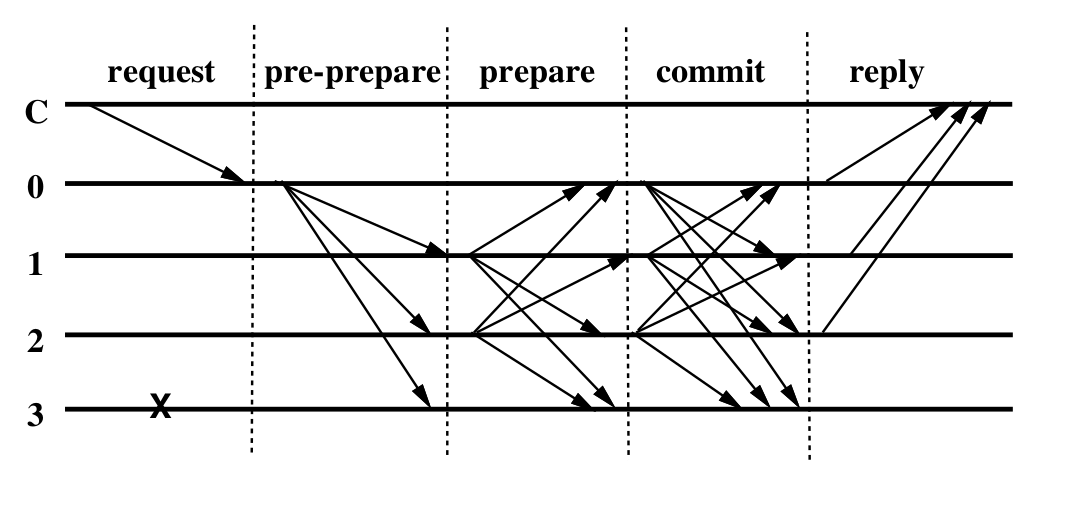
\includegraphics[width=0.75\textwidth]{images/normal-case-op}
    \caption{Resumo da Operação Normal}
  \end{figure}
\end{frame}

\begin{frame}
  \frametitle{Algoritmo}
  \framesubtitle{\textit{Garbage Collection}}

  \begin{itemize}
    \item
      Para garantir \textit{safety}:
      \begin{itemize}
        \item
          Mensagens são mantidas até que a execução de suas requisições por $f + 1$ réplicas corretas possa ser provada;

        \item
          É necessário certificados da corretude do estado.
      \end{itemize}
  \end{itemize}
\end{frame}

\begin{frame}
  \frametitle{Algoritmo}
  \framesubtitle{\textit{Garbage Collection}}

  \begin{itemize}
    \item
      Mecasnismo: \textit{Checkpoints} e \textit{checkpoints} estáveis;

      \pause
    \item
      Réplicas mantêm:
      \begin{itemize}
        \item
          O \textit{checkpoint} estável mais recente;

        \item
          Zero ou mais \textit{checkpoints} não-estáveis;

        \item
          Estado atual.
      \end{itemize}

      \pause
    \item
      Provas são $2f + 1$ mensagens de \textit{checkpoint}.
  \end{itemize}
\end{frame}

\begin{frame}
  \frametitle{Algoritmo}
  \framesubtitle{Mudanças de Visão}

  \begin{itemize}
    \item
      Garante \textit{liveness} permitindo trocar a primária que falhar;

      \pause
    \item
      São ocasionadas por \textit{timeouts};

      \pause
    \item
      Esperas ocorrem quando \textit{backups} recebem requisição ainda não executada.
  \end{itemize}
\end{frame}

\begin{frame}
  \frametitle{Algoritmo}
  \framesubtitle{Mudanças de Visão}

  \textit{Backup} $i$ inicia mudança de visão com mensagem $\braket{\textit{VIEW-CHANGE}, v + 1, n, \mathcal{C}, \mathcal{P}, i}{}_{\sigma_i}$.
  \begin{itemize}
      \pause
    \item
      $n$ é o número de sequência do \textit{checkpoint} estável mais recente que $i$ conhece;

      \pause
    \item
      $\mathcal{C}$ é um conjunto de $2f + 1$ mensagens de \textit{checkpoints} válidas;

      \pause
    \item
      $\mathcal{P}$ é um conjunto de conjuntos $\mathcal{P}_m$ para cada requisição $m > n$ que preparou em $i$:
      \begin{itemize}
        \item
          Mensagem de pré-preparação válida; e
        
        \item
          $2f$ mensagens distintas de preparação correspondentes.
      \end{itemize}
  \end{itemize}
\end{frame}

\begin{frame}
  \frametitle{Algoritmo}
  \framesubtitle{Mudanças de Visão}

  \begin{figure}
    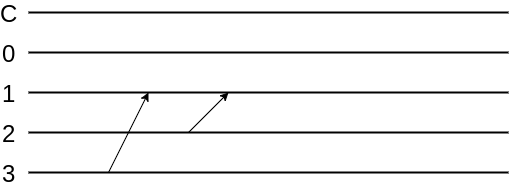
\includegraphics[width=0.75\textwidth]{images/view-change01}<1>
    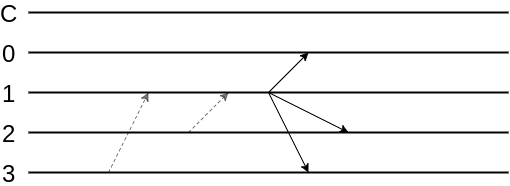
\includegraphics[width=0.75\textwidth]{images/view-change02}<2->
    \only<1>{\caption{Nova primária $p$ recebe $2f$ mensagens de mudança de visão}}
    \only<2->{\caption{$p$ envia $\braket{\text{NEW-VIEW}, v + 1, \mathcal{V}, \mathcal{O}}{}_{\sigma_p}$}}
  \end{figure}
  \pause
  \begin{itemize}
    \item
      $\mathcal{V}$ é uma prova que $2f + 1$ réplicas estão comprometidas com mudança de visão;

      \pause
    \item
      $\mathcal{O}$ é um conjunto de mensagens de pré-preparação para uniformizar os estados das réplicas corretas.
  \end{itemize}
\end{frame}

\begin{frame}
  \frametitle{Algoritmo}
  \framesubtitle{Corretude - \textit{Safety}}

  \textit{Safety} é garantido se réplicas corretas concordam no número de sequência das requisições que possuem \textit{commits} locais.
  \begin{itemize}
    \item
      Invariante (1) garante que se $i, j$ fazem \textit{commits} locais em $v$, então concordam na ordem total;

      \pause
    \item
      Resta provar para réplicas que fazem \textit{commits} locais em visões diferentes.
  \end{itemize}
\end{frame}

\begin{frame}
  \frametitle{Algoritmo}
  \framesubtitle{Corretude - \textit{Safety}}

  \begin{itemize}
    \item
      Um \textit{commit} local de $m$ ocorre se $\texttt{committed}(m, v, n)$ - para $R_1 = f + 1$ réplicas corretas $\texttt{prepared}(m, v, n, i)$;

      \pause
    \item
      Réplicas corretas não aceitam mensagens de pré-preparação para $v' > v$ sem ter recebido mensagem para entrar em $v'$;

      \pause
    \item
      Qualquer mensagem para entrar em $v'$ contém mensagens de mudança de visão de $R_2 = 2f + 1$ réplicas;

      \pause
    \item
      Como $R_1 + R_2 > 3f + 1$, existe $k$ correto tal que $\texttt{prepared}(m, v, n, k)$ e $k$ mudou de visão;

      \pause
    \item
      Mensagem de mudança de visão de $k$ para $v'$ propaga o fato que $m$ for preparada em uma visão anterior.
  \end{itemize}
\end{frame}

\begin{frame}
  \frametitle{Algoritmo}
  \framesubtitle{Corretude - \textit{Liveness}}

  Para garantir \textit{liveness}, réplicas precisam mudar de visão se não conseguem executar uma requisição.
  \begin{itemize}
    \item
      É importante maximizar o tempo em que $2f + 1$ réplicas corretas estão na mesma visão;
      
    \item
      É preciso garantir que esse período aumente exponecialmente.
  \end{itemize}
\end{frame}

\begin{frame}
  \frametitle{Algoritmo}
  \framesubtitle{Corretude - \textit{Liveness}}

  \begin{itemize}
    \item
      \textit{Timers} dobram de duração entre mudanças de visão mal-sucedidas;

      \pause
    \item
      Pedidos de mudança de visão com menor índice são priorizados;

      \pause
    \item
      Réplicas incorretas não podem forçar mudanças de visão frequentemente. No máximo, $f$ réplicas incorretas podem ser primárias consecutivamente.
  \end{itemize}

\end{frame}

\begin{frame}
  \frametitle{Considerações}
  
  \begin{itemize}
    \item
      Algoritmo de replicação de máquina de estados tolerante a falhas bizantinas;

      \pause
    \item
      Funciona em sistemas com suposição fraca de sincronia;

      \pause
    \item
      Artigo descreve otimizações que permitem seu uso na prática e resultados empíricos que fundamentam a afirmação de praticidade.
  \end{itemize}
\end{frame}

\end{document}
